\section{Temperatura obiektu w punkcie pracy}

Zgodnie z poleceniem prowadzącego punkt pracy sterowania ustalono na \num{32}\%.
Sygnał sterujący W1 czyli moc wentylatora ustawiono na \num{50}\%, 
a sygnał sterujący G1 czyli moc grzałki na wyliczone wcześniej \num{32}\% mocy całkowitej.
Następnie przeprowadzono pomiar temperatury w punkcie pracy. 
Uzyskana wartość temperatury punktu pracy wyniosła $\num{36.8}^{\circ} C$.

\begin{figure}[H]
    \centering
    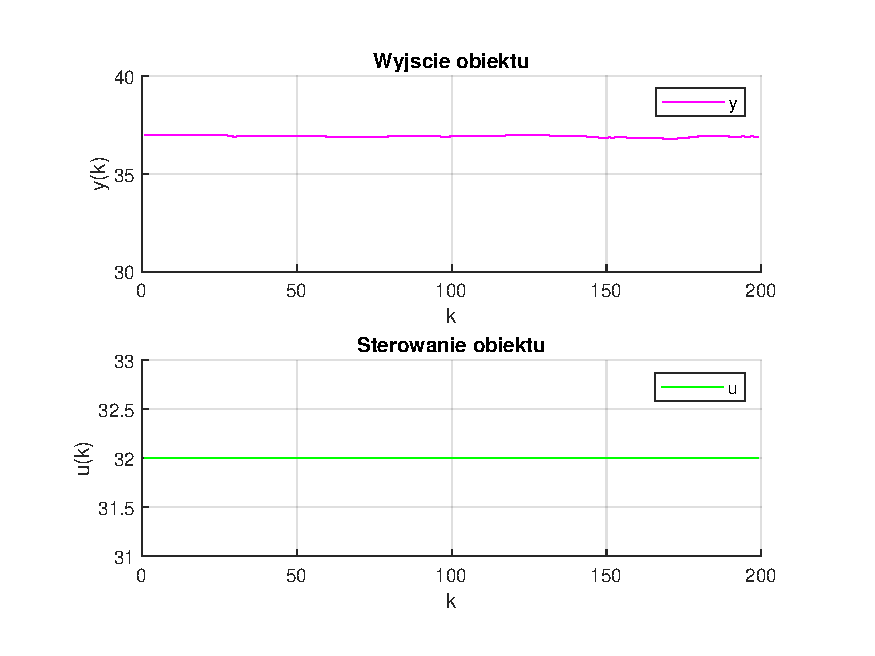
\includegraphics[scale=0.90]{../lab/zad_1/y.pdf}
    \caption{Punkt pracy obiektu}
\end{figure}

